\documentclass[addpoints,11pt]{exam}

\usepackage{alltt}
\usepackage[margin=1in]{geometry}   % set up margins
\usepackage[T1]{fontenc}
\usepackage[usenames,dvipsnames]{xcolor}
\usepackage{enumerate}              % fancy enumerate
\usepackage{amsmath}                % used for \eqref{} in this document
\usepackage{amsthm}
\theoremstyle{definition}
\newtheorem{exmp}{Example}[section]
\usepackage{verbatim}               % useful for \begin{comment} and \end{comment}
\usepackage{eurosym}                % used for euro symbol
\usepackage{caption} 
\usepackage{graphicx}
\graphicspath{{Figures/}}
\usepackage{subcaption}
\usepackage{color}
\usepackage{float}
\usepackage{amssymb}
\usepackage{sgamevar}
\usepackage{sgame}
\usepackage[colorlinks=true]{hyperref}
\hypersetup{colorlinks=true, citecolor=ForestGreen, linkcolor=BlueViolet, urlcolor=Magenta}

%Solutions or nah (blank next two lines out for no solutions, unblank #3)
%\printanswers
%\newcommand{\dd}[1]{\par {\textbf{\textcolor{red}{#1}}}}
\newcommand{\dd}[1]{}  


\setlength\parindent{0pt}
\unframedsolutions
\SolutionEmphasis{\color{red}}
\CorrectChoiceEmphasis{\color{red}}
\renewcommand{\choicelabel}{(\alph{choice})}
\newcommand{\blank}[0]{\underline{\hspace{3cm}}}
\pointformat{\bfseries[\thepoints]}
\pointpoints{pt}{pts}
\pointsinrightmargin


\begin{document}


\title{\textbf{Exam 1} \dd{Solutions} \\ \vspace{2 mm} {\large ECON 101}}
\author{Summer I 2015}
\date{}
\maketitle

\makebox[\textwidth]{Name:\enspace\hrulefill}
\\

\makebox[\textwidth]{ONYEN:\enspace\hrulefill}
\\

\makebox[\textwidth]{PID:\enspace\hrulefill}
\\

\makebox[\textwidth]{Honor Code Signature:\enspace\hrulefill}

\begin{center}
	\fbox{\fbox{\parbox{5.5in}{\centering
				This exam consists of 30 multiple choice questions and 3 short answer questions. Multiple choice questions should be bubbled in on a scantron. Extra paper for scratch work is attached. The total number of points available on this exam is \textbf{100}.}}}
\end{center}



\section*{Multiple Choice [2 pts each]}

Choose the option that best answers the question given.

\begin{questions}
	
	\question You are debating on what to do after this class. Option A is to go watch a baseball game, where tickets cost \$15 a person. On the other hand, you could go watch Mad Max: Fury Road. Tickets at the theater sell for \$10. After stressful exams, you find movies very relaxing and would pay up to \$20 to see this film. Assume there are no other costs to either activity. Based on this, what is your opportunity cost of watching a baseball game this afternoon?
	
		\begin{choices}
				\choice \$15
				\CorrectChoice \$25
				\choice \$35
				\choice \$45
		\end{choices}
		
		
\question Negative externalities lead markets to produce
	
	\begin{choices}
		\choice efficient output levels, and positive externalities lead markets to produce greater than efficient output levels.
		\choice smaller than efficient output levels, and positive externalities lead markets to produce greater than efficient output levels.
		\CorrectChoice greater than efficient output levels, and positive externalities lead markets to produce smaller than efficient output levels.
		\choice greater than efficient output levels, and positive externalities lead markets to produce efficient output levels.
	\end{choices}
	

\question Refer to Figure \ref{MC2}.


\begin{figure}[H]
	\centering
	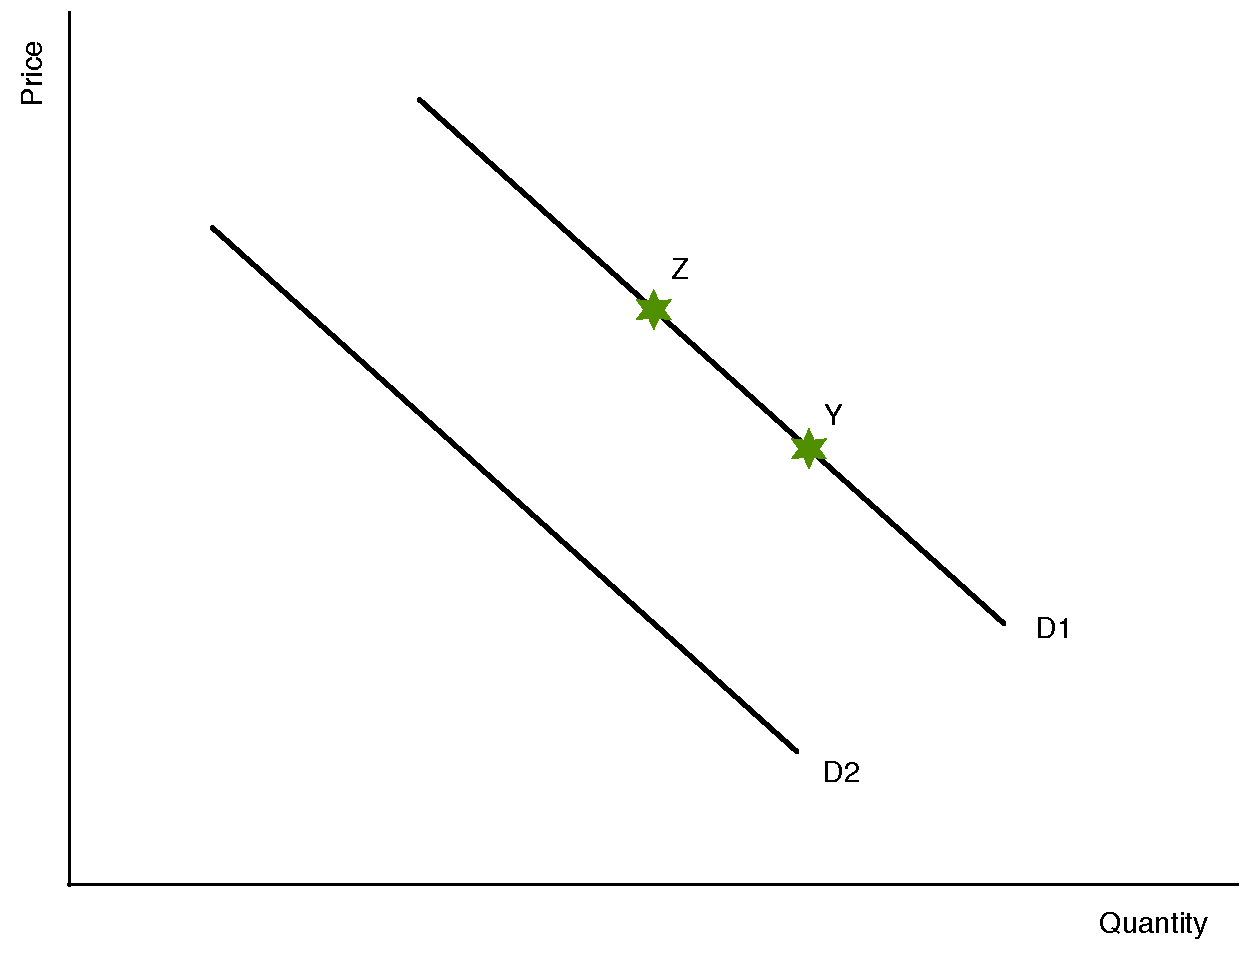
\includegraphics[scale=.40]{Exam1_MC2.pdf}
	\caption{Demand for Shrimp}
	\label{MC2}
\end{figure}

	All else equal, an increase in the income of buyers who consider shrimp to be an inferior good would cause a move from
		
		\begin{choices}
			\choice D2 to D1.
			\choice Y to Z.
			\choice Z to Y.
			\CorrectChoice D1 to D2.
		\end{choices}
		


	\question Suppose demand for pizza shifts such that the market price for pizzas increases. Which of the following statements must be true?
	
		\begin{enumerate}[i.]
			\item Producer surplus increases as existing sellers in the market receive higher prices on the pizzas they were already selling.
			\item New sellers enter the market as a result of the price increase and realize surplus.
			\item Consumer surplus decreases due to the higher price of pizza.
		\end{enumerate}
		
		\begin{choices}
			\choice i and iii
			\CorrectChoice i and ii
			\choice ii and iii
			\choice i, ii, and iii
		\end{choices}

	
	\question The minimum wage in Los Angeles was recently increased from \$9/hour to \$15/hour. This increase in the minimum wage will cause employment to fall by 10\% if \underline{\hspace{3cm}} and results in a(n) \underline{\hspace{3cm}} in wage payments.
	
	\begin{choices}
			\choice labor supply is inelastic; increase
			\CorrectChoice labor demand is inelastic; increase
			\choice labor demand is elastic; decrease
			\choice labor supply is elastic; decrease
	\end{choices}
	
\newpage
	
	\question A non-congested toll road is a \blank because it is \blank.
	
	\begin{choices}
			\CorrectChoice club good; excludable and non-rival
			\choice common resource; excludable and rival
			\choice private good; excludable and rival
			\choice public good; non-excludable and non-rival
	\end{choices}

	
	\question Consultants hired by Sunnyside Eggs find that the firm has total fixed costs of \$50,000, total variable costs of \$25,000, and total revenues of \$40,000. Given this, in the short run the firm should \blank and make \blank profit.
	
	\begin{choices}
		\choice shut down; negative
		\choice shut down; zero
		\CorrectChoice stay open; negative
		\choice stay open; positive
	\end{choices}

		
\uplevel{Use Table \ref{MC8}, which shows the quantity of belts and shoes that Hank and George can produce per hour, to answer questions \ref{q8} - \ref{q10}.}
	
	\begin{table}[ht]
		\caption{Production of Belts and Shoes (per hour)}
		\centering
		\begin{tabular}{  c| c c} 
			
			& Hank & George \\
			\hline
			Belts & 4 & 6 \\
			Shoes & 12 & 6 \\
		\end{tabular}
		\label{MC8}
	\end{table}

	
\question \label{q8} Given this information, it follows that 

\begin{choices}
	\choice Hank has an absolute advantage in the production of belts, while George has an absolute advantage in the production of shoes.
	\choice Hank has an absolute advantage in the production of both belts and shoes.
	\CorrectChoice Hank has an absolute advantage in the production of shoes, while George has an absolute advantage in the production of belts.
	\choice George has an absolute advantage in the production of both belts and shoes.
\end{choices}

\question \label{q9} From the information, we can also discern that Hank has a comparative advantage in 

\begin{choices}
	\choice both goods, and George has a comparative advantage in neither good.
	\choice belts, and George has a comparative advantage in shoes.
	\choice neither good, and George has a comparative advantage in both goods.
	\CorrectChoice shoes, and George has a comparative advantage in belts.
\end{choices}


\question \label{q10} Which of the following terms of trade, if any, would make both Hank and George better off?

\begin{choices}
	\CorrectChoice 200 belts per 400 shoes
	\choice 100 belts per 400 shoes
	\choice 66 shoes per 100 belts
	\choice None of the above
\end{choices}
	

	\question Chocolate chip cookies and oatmeal raisin cookies are substitutes. If the price of chocolate chip cookies increases, then the equilibrium price of oatmeal cookies will \blank and the equilibrium quantity will \blank.
	
	\begin{choices}
			\choice increase; decrease
			\choice decrease; increase
			\CorrectChoice increase; increase
			\choice decrease; decrease
	\end{choices}
	


	\question Since chocolate chip cookies and oatmeal raisin cookies are substitutes, the cross-price elasticity of demand between the goods is 
	
	\begin{choices}
		\choice negative.
		\CorrectChoice positive.
		\choice zero.
		\choice impossible to discern without more information.
	\end{choices}
	

\question A market is currently at equilibrium. A price ceiling above the equilibrium price is imposed, leading to \underline{\hspace{3cm}} in producer surplus and \underline{\hspace{3cm}} in total surplus.
	
	\begin{choices}
			\choice a decrease; an increase
			\choice an increase; an increase
			\choice a decrease; a decrease
			\CorrectChoice no change; no change
	\end{choices}
	

	
\question In order to maximize profit, a firm in a perfectly competitive market will produce at the quantity where

\begin{choices}
	\CorrectChoice $AR = MC$.
	\choice $P = ATC$.
	\choice $P = AVC$.
	\choice $MR = ATC$.
\end{choices}

	
\question  A neighborhood street is considering purchasing and installing doggy clean up stations in order to keep their lawns clean. Table \ref{MC15} shows the willingness to pay of each family for each station.

\begin{table}[ht]
	\caption{Willingness to Pay for Doggy Stations}
	\centering
	\begin{tabular}{  c| ccc} 
		
		Stations & Weiners Family & George Family & Heron Family\\
		\hline
		1st station & \$500 & \$600 & \$400\\
		2nd station & 400 & 450 & 300\\
		3rd station & 300 & 350 & 150\\
		4th station & 150 & 200 & 50\\
		5th station & 100 & 150 & 0\\
	\end{tabular}
	\label{MC15}
\end{table}

\newpage

If each doggy station costs \$500, how many stations should the street install in order to maximize total surplus?
	
	\begin{choices}
			\choice 2 stations
			\choice 0 stations
			\CorrectChoice 3 stations
			\choice 1 stations
	\end{choices}
	
		
\question Refer to Figure \ref{MC16}, which shows the market for laptop computers.

\begin{figure}[H]
	\centering
	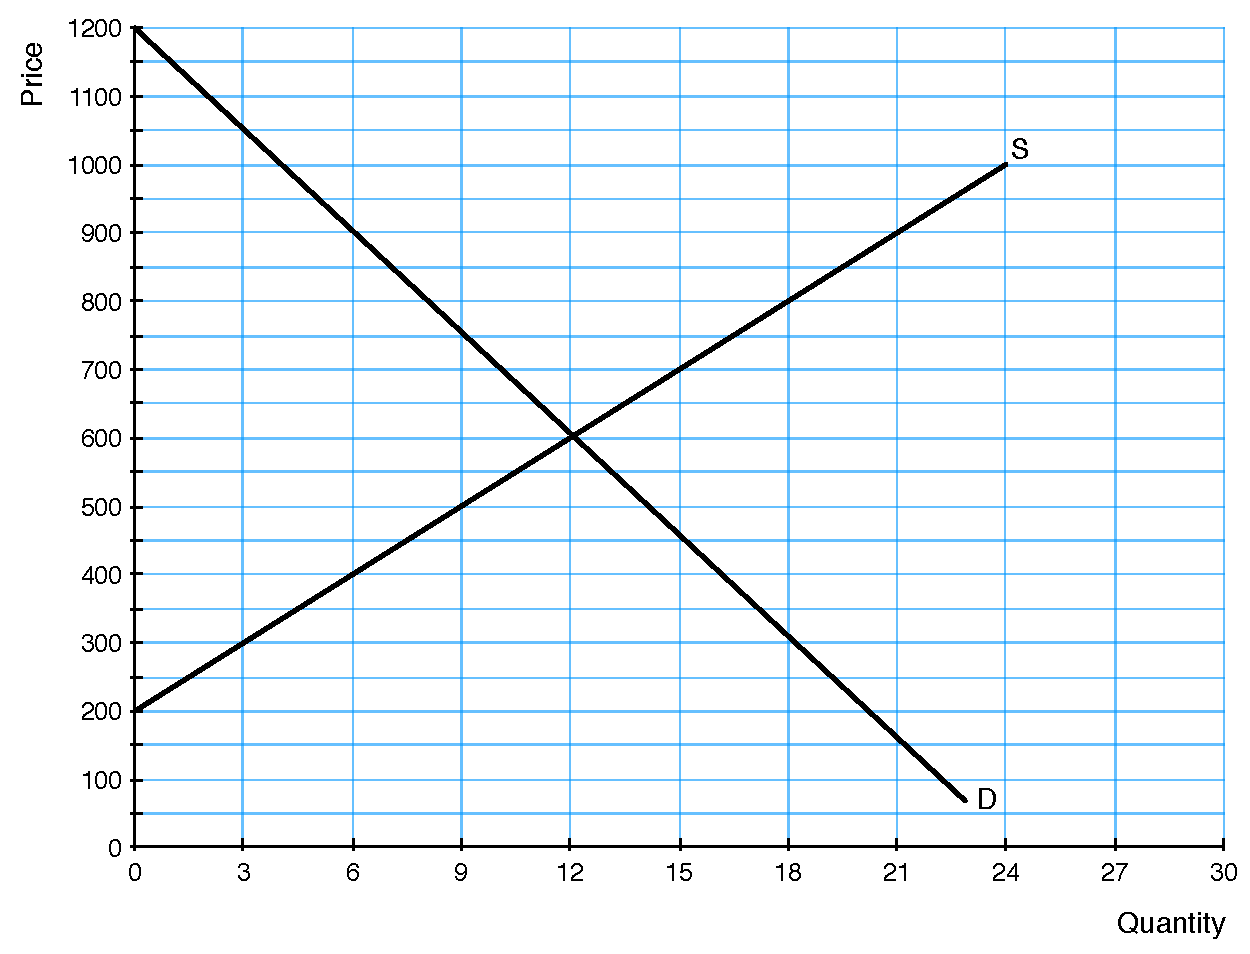
\includegraphics[scale=.40]{Exam1_MC16.pdf}
	\caption{Market for Laptops}
	\label{MC16}
\end{figure}

If a tax of \$500 is imposed on buyers, then the share of the tax bore by consumers is

	\begin{choices}
			\choice \$200.
			\CorrectChoice \$300.
			\choice \$500.
			\choice \$900.
	\end{choices}
	

	
	\question Table \ref{MC17} shows the quantity supplied and demanded at certain prices.
	
	
	\begin{table}[h!]
		\caption{Prices and Quantities}
		\centering
		\begin{tabular}{  c | c | c} 
			
			Price & $Q_d$ & $Q_s$ \\
			\hline
			\$10 & 50 & 30 \\
			\$12 & 45 & 35 \\
			\$14 & 40 & 40 \\
			\$16 & 35 & 45 \\
			\$18 & 30 & 50 \\
		\end{tabular}
		\label{MC17}
	\end{table}
	
\newpage
	
	If the price in the market were \$12, there would be
	
	\begin{choices}
			\CorrectChoice a shortage of 10 units.
			\choice a surplus of 35 units.
			\choice a shortage of 45 units.
			\choice a surplus of 10 units.
	\end{choices}
	


	\question Bluth's Bananas currently employs 5 workers and produces 1,000 frozen bananas a day. In preparation for the busy summer season, the firm is debating whether they should hire 5 more workers. If they do, they project they could produce 1,500 frozen bananas a day. Given this, the marginal product of labor per worker from these additional workers would be
	
	
	\begin{choices}
			\choice 1,500.
			\choice 500.
			\choice 150.
			\CorrectChoice 100.
	\end{choices}
	

	
	\question Consider Figure \ref{MC19}. 
	
	\begin{figure}[H]
		\centering
		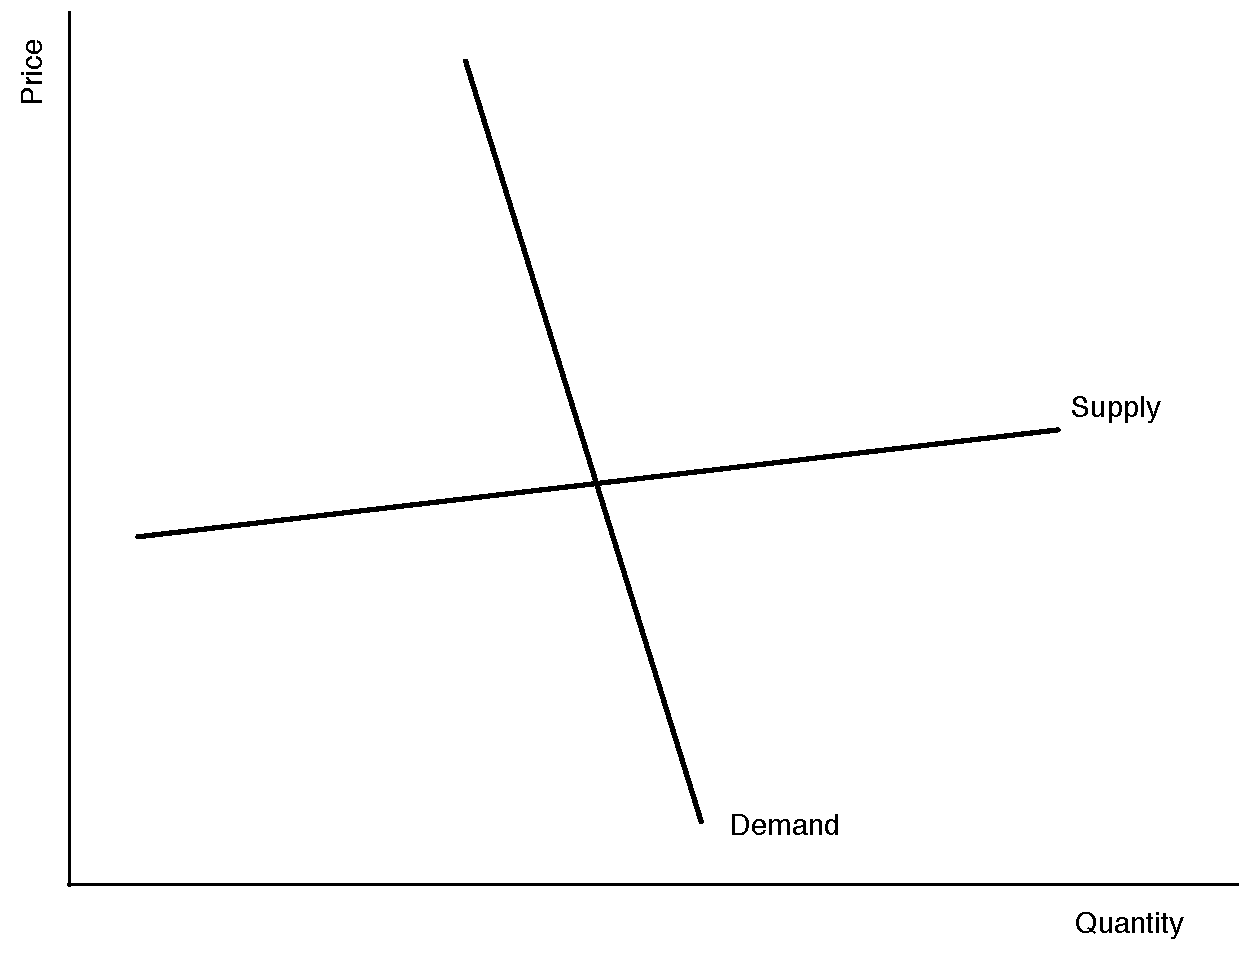
\includegraphics[scale=.40]{Exam1_MC19.pdf}
		\caption{Market for Coke}
		\label{MC19}
	\end{figure}
	
	If the government imposes a \$5 per unit tax on sellers in this market,  
	
	\begin{choices}
		\choice the burden of the tax will be split evenly between buyers and sellers in the market.
		\choice the burden of the tax will be greater for sellers than for buyers in the market.
		\CorrectChoice the burden of the tax will be greater for buyers than for sellers in the market.
		\choice the split of the tax burden cannot be determined from this information. 
	\end{choices}
	
\newpage
	
	\question The opportunity cost of attending college does \textbf{not} include
	
	\begin{choices}
		\choice the potential salary you could earn by quitting school and working now.
		\choice the costs of room and board, books, and class materials.
		\CorrectChoice the potential salary you could earn after finishing your degree.
		\choice the psychological costs of stress and lack of sleep.
	\end{choices}

	
	\question As individuals lose their jobs, they buy fewer romance novels. Which of the following might be the income elasticity of demand for romance novels?
	
	\begin{choices}
		\choice $-1.32$
		\CorrectChoice $.54$
		\choice $-.30$
		\choice Either (a) or (c)
	\end{choices}

	
	\question The United States currently produces guns and butter. Table \ref{MC22} shows possible combinations of the two goods the US can produce in a given week (in thousands). 
	
	\begin{table}[h!]
		\caption{Weekly Production of Guns and Butter}
		\centering
		\begin{tabular}{  c| c} 
			
			Guns & Butter \\
			\hline
			5 & 50 \\
			10 & $x$  \\
			15 & 30 \\
		\end{tabular}
		\label{MC22}
	\end{table}
	
	If resources in the US are specialized such that some are better suited to producing guns and others are better suited for butter production, then a possible value for $x$ might be
		
		\begin{choices}
				\choice 30
				\choice 35
				\choice 40
				\CorrectChoice 45
		\end{choices}
		
	
	
	\question Figure \ref{MC23} shows the demand curve for Fanta.
	
	\begin{figure}[H]
		\centering
		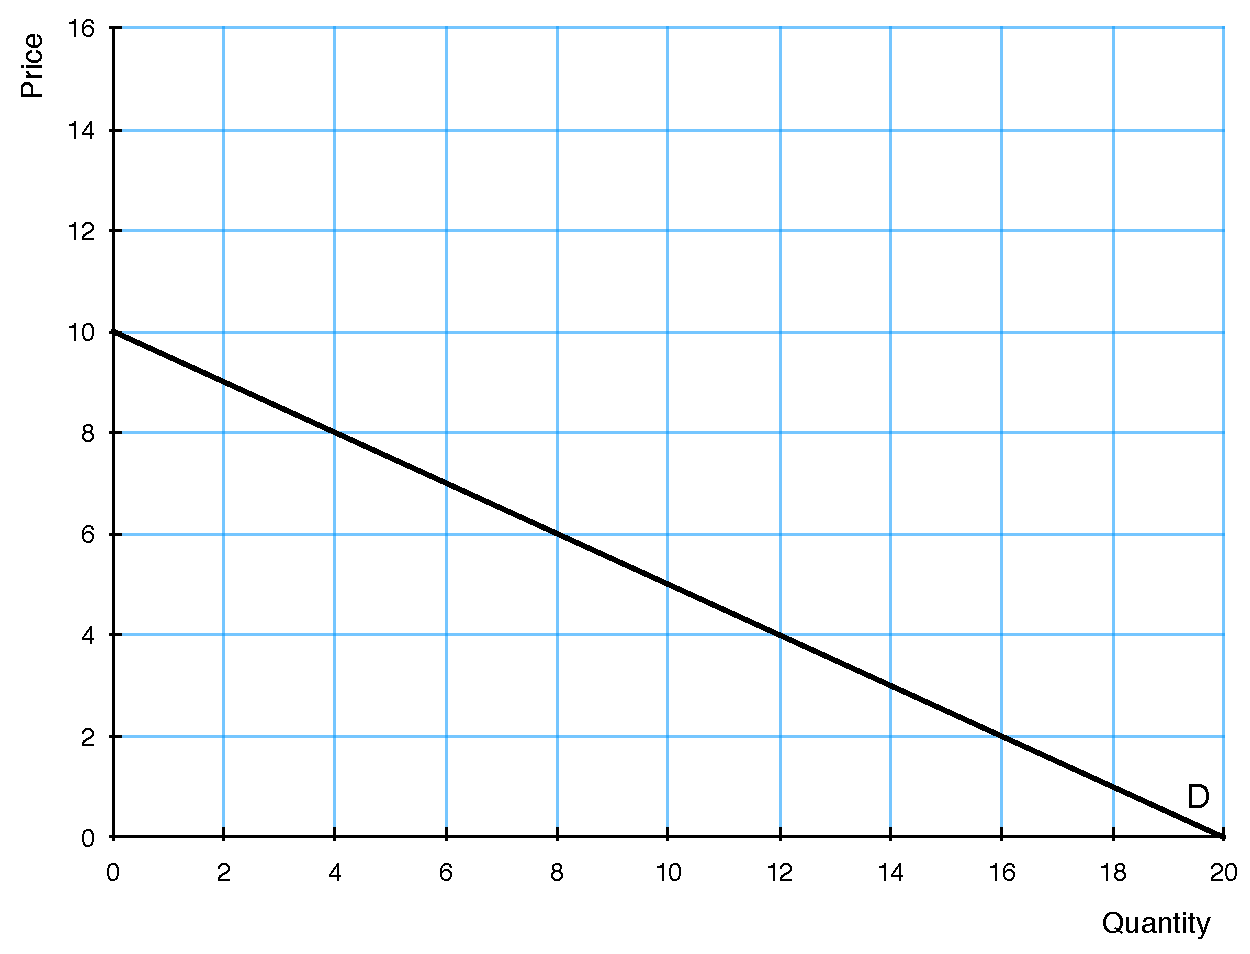
\includegraphics[scale=.40]{Exam1_MC22.pdf}
		\caption{Demand for Fanta}
		\label{MC23}
	\end{figure}
	
	If the price of Fanta decreases from \$8 to \$4, the increase in consumer surplus that is realized by new buyers entering the market due to the price decrease is 
	
	\begin{choices}
			\choice \$36.
			\choice \$32.
			\CorrectChoice \$16.
			\choice \$8.
	\end{choices}
	
	
	\question If the price elasticity of supply is .8, and prices increased by 5\%, then quantity supplied would
	


	\begin{choices}
		\CorrectChoice increase by 4\%.
		\choice decrease by 4\%.
		\choice increase by 6.25\%.
		\choice decrease by 6.25\%.
	\end{choices}

	
	\question Suppose the demand for single family homes increases due to a decline in interest rates. At the same time, a major home builder goes bankrupt and no longer builds homes. As a result, the equilibrium quantity of single family homes
	
	\begin{choices}
		\choice increases, while the equilibrium price of homes decreases.
		\CorrectChoice changes ambiguously, while the equilibrium price of homes increases. 
		\choice decreases, while the equilibrium price of homes increases.
		\choice increases, while the equilibrium price of homes changes ambiguously.
	\end{choices}
	
		
\question Consider Figure \ref{MC25}. 

\begin{figure}[H]
	\centering
	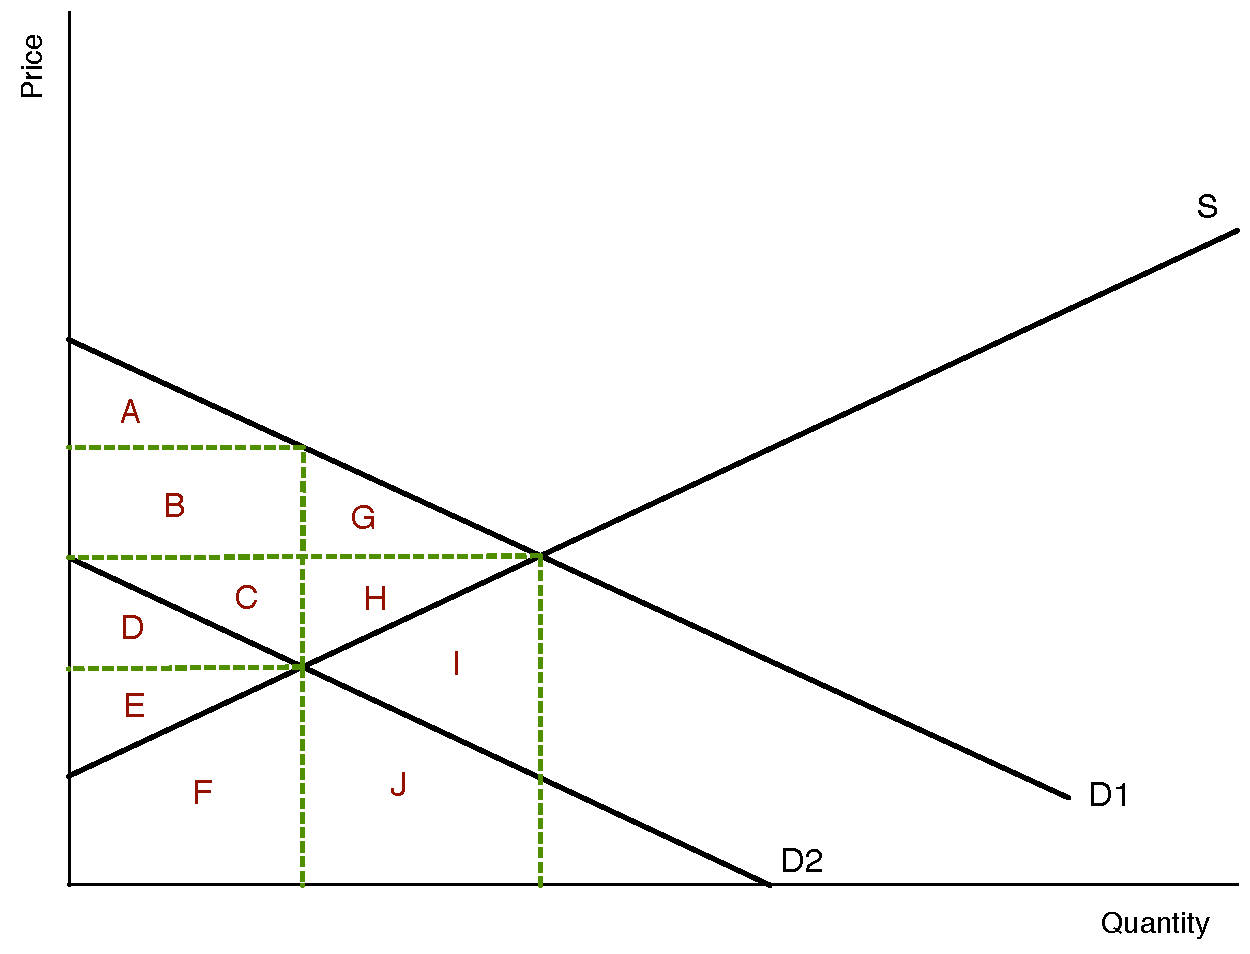
\includegraphics[scale=.40]{Exam1_MC25.pdf}
	\caption{Market for Fanta}
	\label{MC25}
\end{figure}

\newpage

If demand is originally given by D2, and then shifts to D1, total surplus in the market

\begin{choices}
	\choice increases by areas A+B+C+G+H+I
	\choice increases by areas A+B+C+D+E+G+H
	\choice increases by areas A+B+C+D+E
	\CorrectChoice increases by areas A+B+C+G+H
\end{choices}



\question A tax of \$4 is imposed by the government. Use Table \ref{MC27} to answer the question below.

\begin{table}[h!]
	\caption{Unit Taxes}
	\centering
	\begin{tabular}{  c| c | c} 
		
		& Price with no tax & Price with \$4/unit tax on sellers \\
		\hline
		Price paid by buyers & \$55 & ? \\
		Price paid by sellers & \$55 & \$53.50  \\
	\end{tabular}
	\label{MC27}
\end{table}

Because of this tax, buyers are paying \underline{\hspace{3cm}} per unit and sellers are receiving \underline{\hspace{3cm}} per unit.

\begin{choices}
		\choice \$4 less; \$4 more
		\choice \$2 more; \$2 less
		\CorrectChoice \$2.50 more; \$1.50 less
		\choice \$4 more; \$4 less
\end{choices}


	
	\question Al's Burgers is a firm in a competitive market and faces the cost structure shown in Figure \ref{MC28}.
	
	\begin{figure}[H]
		\centering
		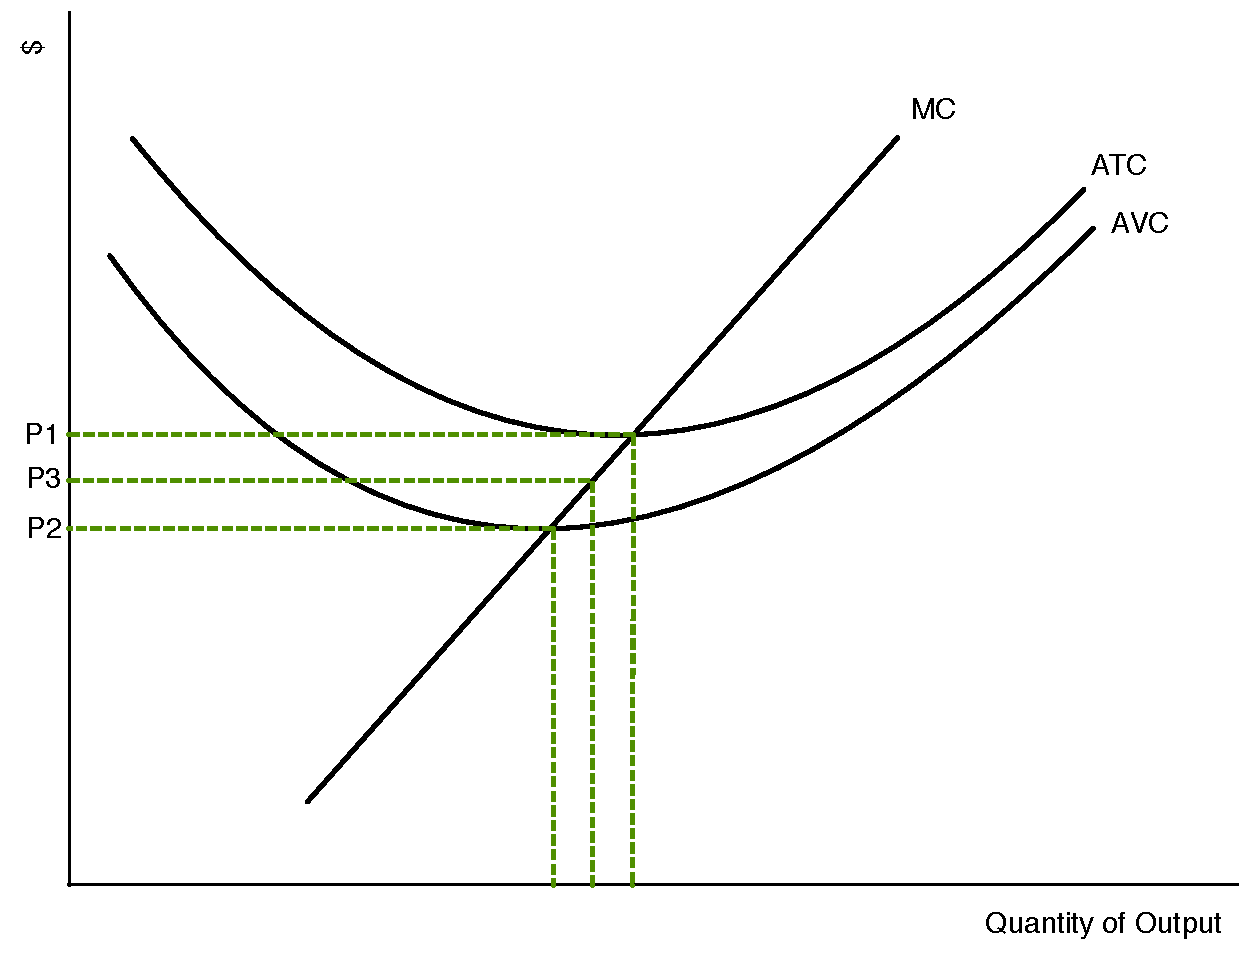
\includegraphics[scale=.40]{Exam1_MC27.pdf}
		\caption{Market for Fanta}
		\label{MC28}
	\end{figure}
	
\newpage
	
	The firm decides to operate in the short run, but incurs economic losses. Thus, the market price must be 

	\begin{choices}
		\choice less than P2.
		\choice greater than P2 but less than P3.
		\choice greater than P3 but less than P1.
		\CorrectChoice greater than P2 but less than P1.
		\choice greater than P1.
	\end{choices}

	
\question A firm currently produces 1,000 units of output with an average variable cost of \$5.10. The firm has fixed costs of \$5,000. If the firm were to produce 1,001 units, its total variable costs would be \$5,400. What is the marginal cost to the firm of producing 1,001 units?
		
		
		\begin{choices}
			\choice \$5,400
			\CorrectChoice \$300
			\choice \$5,100
			\choice \$400
		\end{choices}

	
	\question Matthew is trying to determine how many sticks of RAM he should buy for his computer. Each additional stick increases the speed of his computer by 50\%. On a typical day, he would be willing to pay \$100 for each 50\% increase in computing power. The total costs of acquiring and installing each stick of RAM are detailed in Table \ref{MC30}. 
	
	\begin{table}[h!]
		\caption{Total Costs of RAM}
		\centering
		\begin{tabular}{ c| c} 
			
			Sticks of RAM &  Total Cost\\
			\hline
			1 & \$50 \\
			2 & \$100  \\
			3 & \$175 \\
			4 & \$300 \\
			5 & \$600 
		\end{tabular}
		\label{MC30}
	\end{table}
	
	How many sticks of RAM should Matthew purchase?
	
	\begin{choices}
		\choice 1
		\choice 2
		\CorrectChoice 3
		\choice 4
	\end{choices}
	

\end{questions}

\newpage

\section*{Short Answer}

For this section, make sure to write legibly and box final answers. \textbf{Show your work!} This can be done within the section or \textit{clearly} labeled on the scratch paper provided.

\begin{questions}


	\question Consider Figure \ref{SA1}, which reflects the market for Surface Tablets in United States.
	
	\begin{figure}[H]
		\centering
		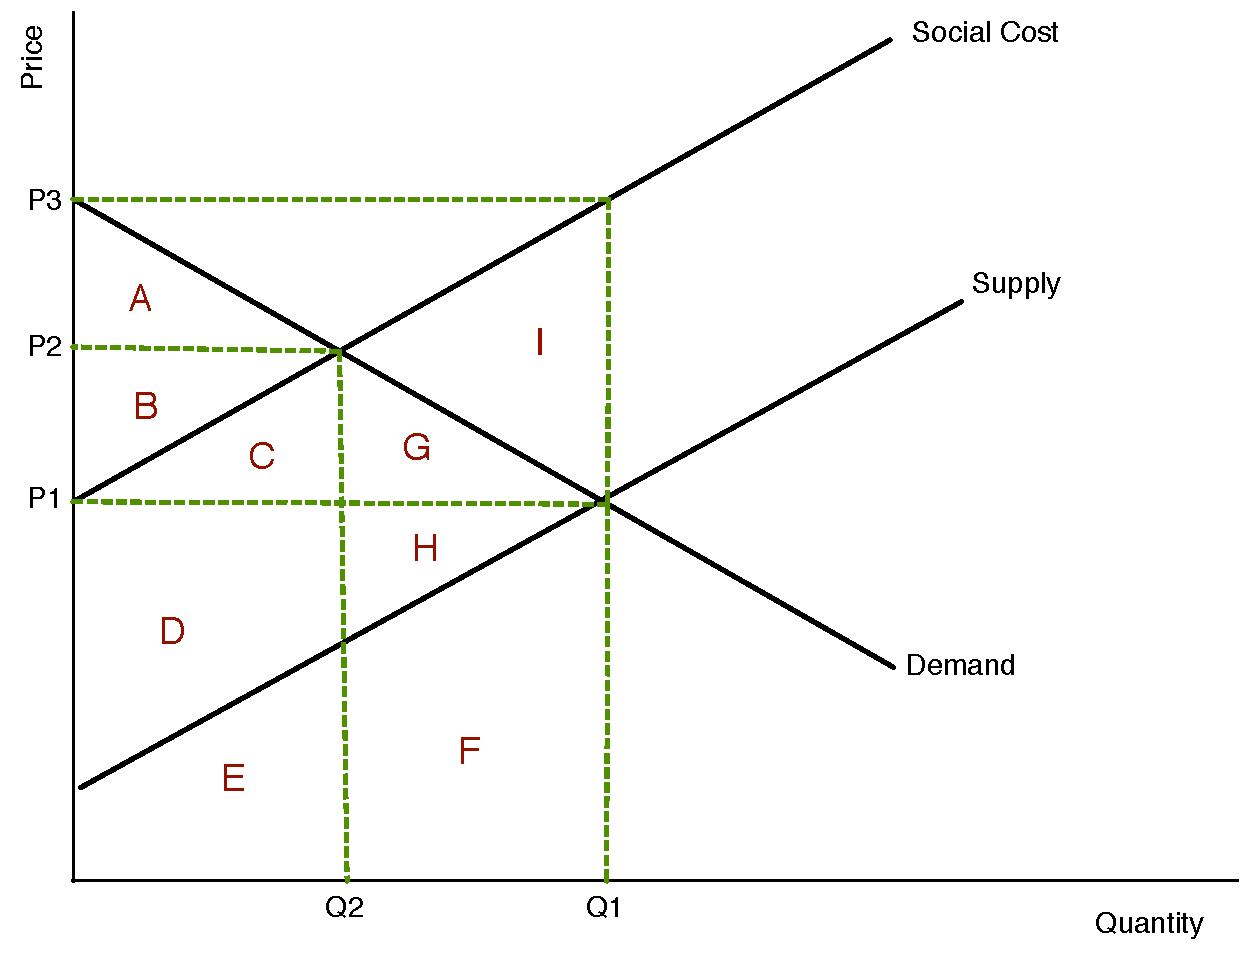
\includegraphics[scale=.45]{Exam1_SA1.pdf}
		\caption{Market for Surface Tablets}
		\label{SA1}
	\end{figure}
	
	\begin{parts}
		\part[2] What price and quantity combination represents the market price and number of units produced? 
		\vspace{1cm}		 
	
		
		\part[2] At the market quantity, what area (or combination of areas) represents the total external cost to society?
		\vspace{1cm}		 
		
		\part[2] What is the social optimum quantity of Surface Tablets that should be produced?
		\vspace{1cm}		 		

		\part[2] At the social optimum, what area (or combination of areas) represents the total surplus realized by society? 
		\vspace{1cm}		 
				
		\part[2]  A policy advisor suggests that in order to reach the social optimum point, a tax of ($P3 - P2$) should be imposed. Do you agree or disagree? Why?
		\vspace{1cm}		 		
		
	\end{parts}
	
	
\newpage
	
	\question Table \ref{SA2} shows the willingness to pay and costs of five sellers and buyers in the market for new textbooks. Each buyer would like one textbook and each seller has one book to sell. 
	
	\begin{table}[ht]
		\caption{WTP and Seller Costs for Textbooks}
		\centering
		\begin{tabular}{  c| c} 
			
			WTP   & Seller Costs \\
			\hline
			\$180 & \$85 \\
			\$150 & \$150 \\
			\$100 & \$100 \\
			\$200 & \$125 \\
			\$125 & \$60 \\
		\end{tabular}
		\label{SA2}
	\end{table}
	
	
	
	Use the table to answer the following questions.
	
	\begin{parts}
		\part[4] If the market price is currently \$110, is there a shortage or a surplus? Explain. What do you expect will happen to the market price?
		\vspace{1.5cm}
		
		
		\part[2] What is the market equilibrium price and quantity in this market?
		\vspace{1cm}
		
		\part[2] At the market equilibrium, what is the total surplus realized?
		\vspace{1cm}
		
		\part[3] Under pressure from textbook sellers, the government passes a law that the price of textbooks can go no lower than \$120. What is the market price and quantity exchanged as a result of this law?
		\vspace{1.5cm}
		
		\part[3] Suppose the demand curve for textbooks shifted such that each buyer values a textbook \$50 less than before. The law outlined in (d) is still in place. What is the market price and quantity exchanged? What is the consumer surplus realized?
		\vspace{1.5cm}
		
	\end{parts}
	
	\question A firm is considering whether to enter a perfectly competitive market, with the conditions outlined in Table \ref{SA3}. By entering the market, the firm would have to pay fixed costs of \$900 per day.
	
	\begin{table}[H]
		\caption{Market Environment}
		\centering
		\begin{tabular}{ c| c | c | c | c} 
			
			Quantity (per day)   & Marginal Revenue &  Marginal Cost & Variable Costs & Total Costs\\
			\hline
			1 & \$750 &  \$150 & &\\
			2 & \$750 & \$400 && \\
			3 & \$750 & \$750 && \\
			4 & \$750 & \$1,250&& \\
		\end{tabular}
		\label{SA3}
	\end{table}
	
	Use this information to answer the following questions.
	
	\begin{parts}
		\part[2] What is the market price the firm would receive for every unit of output it sold? 
		\vspace{.5cm}
		\part[4] Fill in the column labeled ``Variable Costs.'' 
		\part[2] Fill in the column labeled ``Total Costs.'' 
		\part[2] What would be the level of production the firm would operate at were it to enter the market?
		\vspace{1cm}
		\part[4] Should this firm enter the market? Explain why. 
		\vspace{1.5cm}
		\part[2] What would be the firm's profits per day if it entered the market?
		\vspace{1cm}
	\end{parts}
	
\end{questions}

\hrulefill
\begin{center} 
	\textbf{END OF EXAM}
\end{center}

\newpage

\centering

\section*{SCRATCH SHEET}



\end{document}